\subsection{Sensitivity analysis}
\begin{frame}
    \frametitle{Sensitivity analysis provides more insight into 
    the fuel cycles.}
    To meet the third objective, I perform sensitivity analysis 
    on Scenario 7, comparing the impact of different model parameters
    \begin{itemize}
        \item Couple \Cyclus with Dakota \cite{adams_dakota_2021}
        \item Parameters include:
        \begin{itemize}
            \item Transition start time
            \item Percent of \glspl{LWR} operating for 80 years
            \item Build share of Xe-100, VOYGR, MMR
            \item Discharge burnup of Xe-100 and MMR
        \end{itemize}
        \item Vary these parameters individually
        \item Vary these parameters in different combinations
    \end{itemize}

\end{frame}

\begin{frame}
    \frametitle{Varying the Xe-100 build share has a mixed effect}
    \begin{columns}

        \column[t]{4.5cm}
        \begin{itemize}
            \item HALEU-related metrics all increase
            \item Total fuel mass and the SNF mass decrease
            \item Total SWU capacity is relatively constant
            \item Results are a function of the number of
                  each advanced reactor deployed
        \end{itemize}

    \column[t]{5.5cm}
    \begin{figure}
        \centering 
            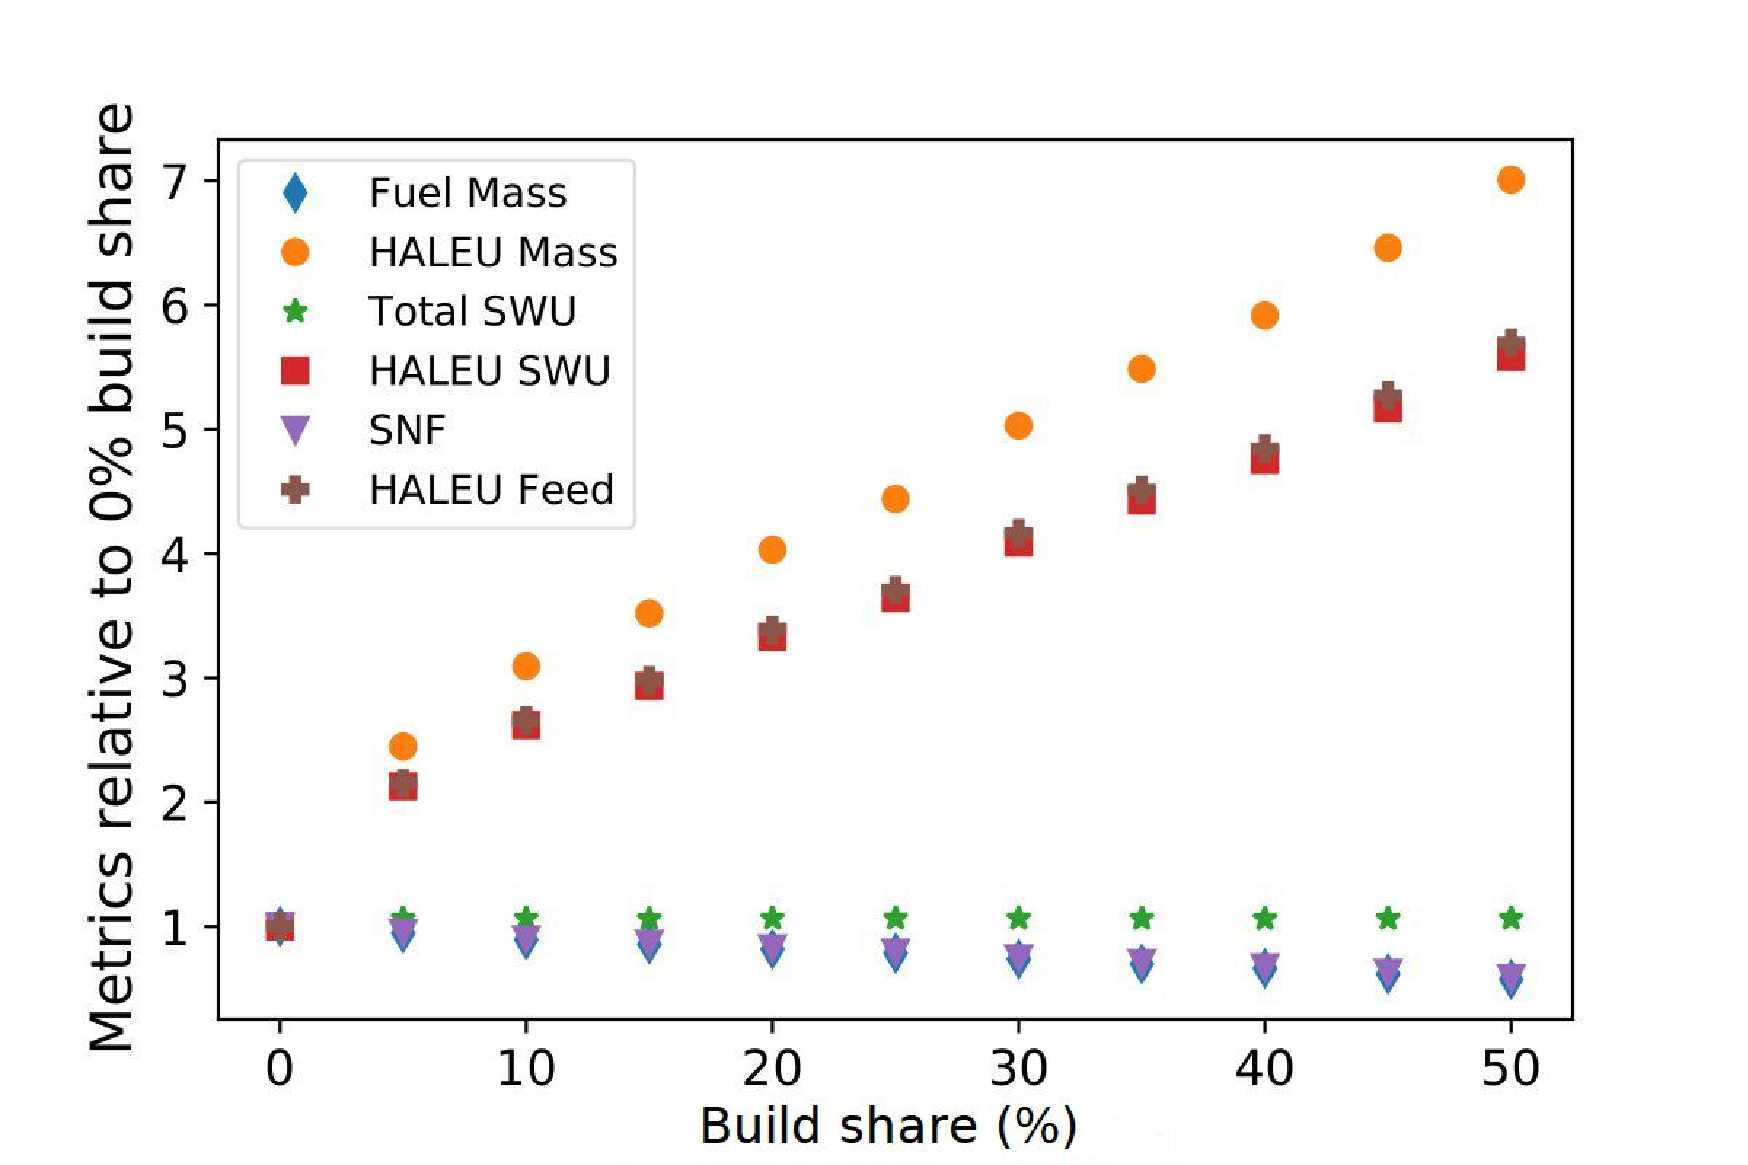
\includegraphics[scale=0.4]{xe100.pdf}
            \caption{Relative effect of varying Xe-100 build share}
            \label{fig:xe100_effects}
    \end{figure}

\end{columns}
\end{frame}

\begin{frame}
    \frametitle{Effects of varying Xe-100 build share}
    \begin{figure}
        \centering
        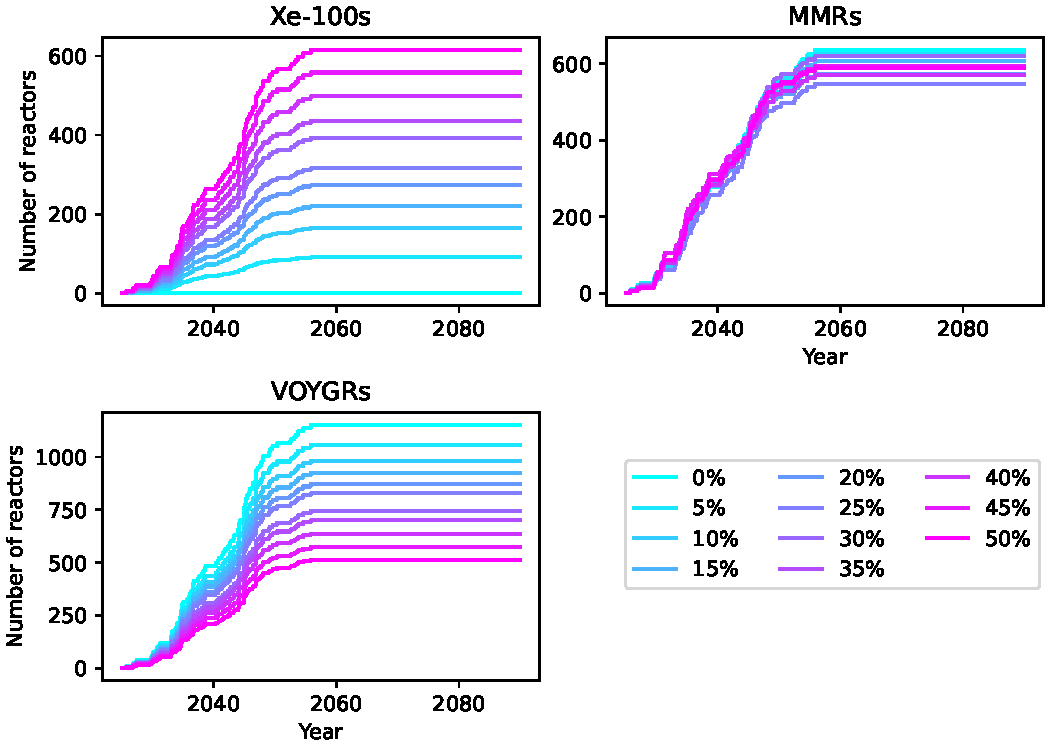
\includegraphics[scale=0.5]{xe100_combined_reactors.pdf}
        \caption{Number of Xe-100s (top left), MMRs (top right), and VOYGRs
        (bottom left) as a function of Xe-100 build share.}
        \label{fig:xe100_s7_combined_reactors}
    \end{figure}
\end{frame}

\begin{frame}
    \frametitle{Effects of varying Xe-100 and MMR burnup}
    \begin{columns}

        \column[t]{4cm}
        \begin{itemize}
            \item Non-uniform relationship
            \item At smaller Xe-100 burnup values the increasing MMR 
                  share decreases the HALEU mass
            \item At larger Xe-100 burnup values the increasing MMR share 
                  increases the HALEU mass
            \item Comparison of how much fuel each reactor needs
        \end{itemize}

    \column[t]{6cm}
    \vspace{-1cm}
    \begin{figure}
        \centering 
            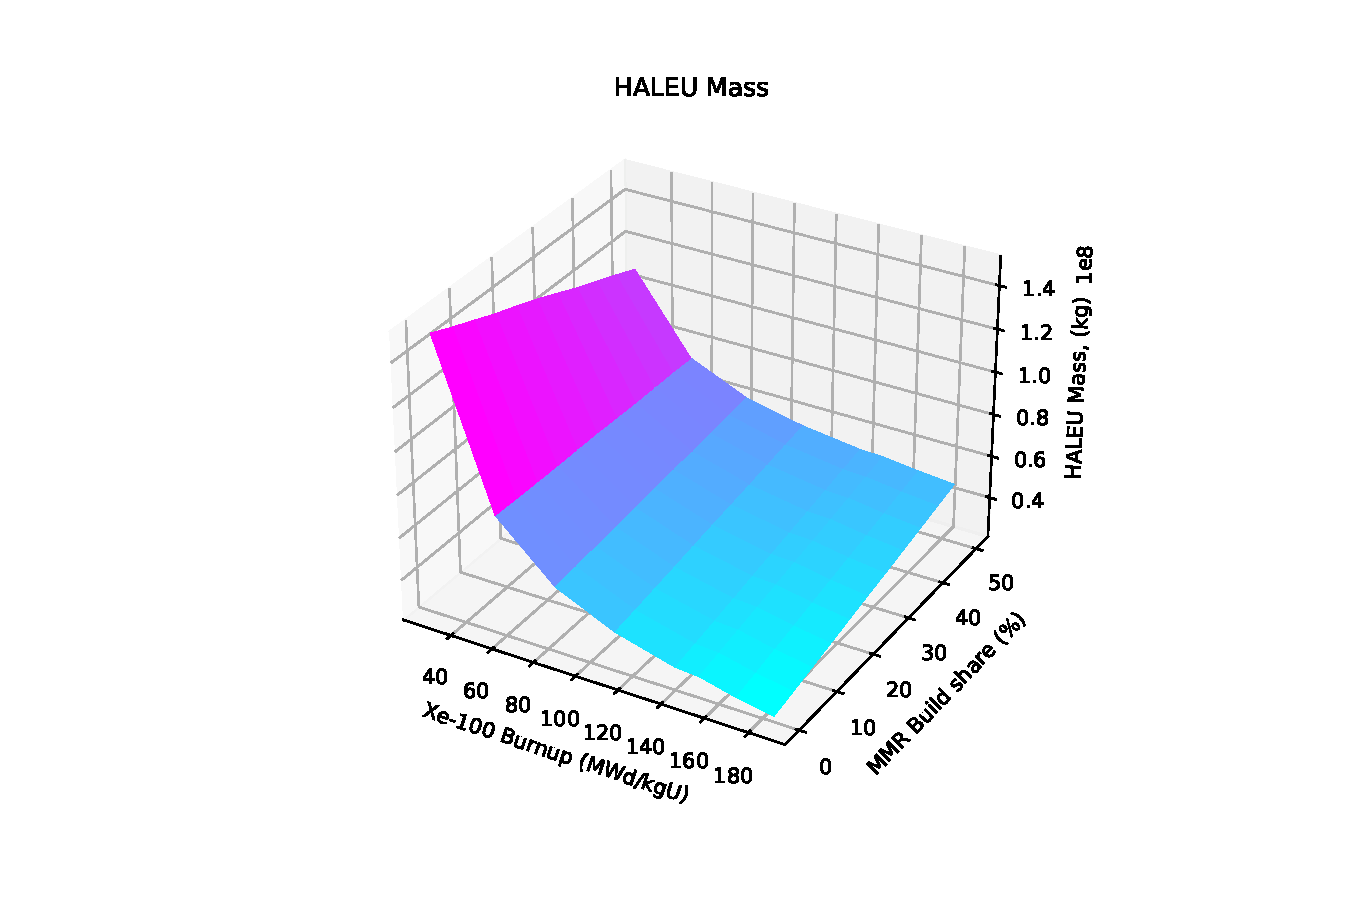
\includegraphics[scale=0.5, trim=180 45 70 50,clip]{mmr_share_xe100_burnup_haleu.pdf}
            \caption{Effects of varying the MMR build share and 
            Xe-100 discharge burnup on HALEU mass}
            \label{fig:mmr_share_xe100_bu}
    \end{figure}

\end{columns}
\end{frame}

\begin{frame}
    \frametitle{Varying multiple parameters shows importance of the 
    Xe-100 burnup}
    \begin{table}
        \centering
        \caption{Sobol' indices for the Gaussian model when varying the 
        Xe-100 build share. Highlighted 
        values indicate a total Sobol' indices of above 0.5.}
        \label{tab:s7_sobol_xe100_gaussian}
        \begin{tabular}{c c c c c c c}
            \hline
            & \multicolumn{6}{c}{Output Metric} \\
            Parameter & Fuel Mass & HALEU Mass & SWU & HALEU SWU & Feed & SNF Mass \\
            \hline
            Transition Start & 0.003 & 0.007 & 0.009 &
                               0.009 & 0.009 & 0.003\\
            LWR Lifetime & 0.280 & 0.021 & 0.095 &
                           0.022 & 0.022 & 0.314\\
            Xe-100 Share & \cellcolor{green!25}0.533 & \cellcolor{green!25}0.513 & 0.283 &
            \cellcolor{green!25}0.511 & \cellcolor{green!25}0.512 & 0.474\\
            Xe-100 Burnup & 0.247 & \cellcolor{green!25}0.571 & \cellcolor{green!25}0.775 & 
            \cellcolor{green!25}0.568 & \cellcolor{green!25}0.568 & 0.280\\
            MMR Burnup & 0.002 & 0.004 & 0.006 & 
                         0.005 & 0.005 & 0.002\\
            \hline        
        \end{tabular}
    \end{table}
        %<2-> \tikz[overlay, remember picture]{\draw{draw=red,thick, double, fillopacity=0.2] ($(infrastructure)+(-0.5,0.4)$) rectangle ($(infrastructure)+(6,-0.2)$);}} 
\end{frame}

\subsection{Optimization}
\begin{frame}
    \frametitle{Use the \Cyclus-Dakota coupling to optimize the transition}
    \begin{itemize}
        \item Use the Genetic algorithm in Dakota (single-objective or 
        multi-objective) to perform optimization.
        \item Use the parameters considered for sensitivity analysis, 
              except the transition start time
        \item Apply a linear constraint for the advanced reactor build shares
        \item Goal is to minimize the SWU capacity needed to 
             produce HALEU, the mass of SNF, or both
    \end{itemize}
\end{frame}

\begin{frame}
    \frametitle{Multi-objetive optimization isn't perfect}
    \begin{columns}
        \column[t]{5cm}
        \begin{itemize}
            \item Optimizing for these metrics is a trade-off between 
                 building Xe-100s and VOYGRs
            \item Genetic algorithm struggles with linear constraint for 
                  the three build shares
        \end{itemize}

        \column[t]{5cm}
        \begin{figure}
            \centering 
            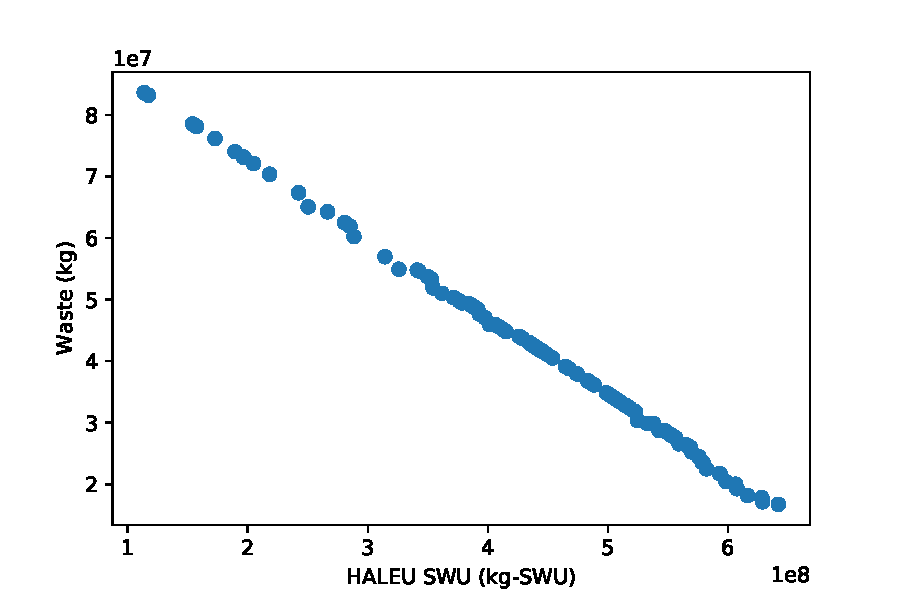
\includegraphics[scale=0.4]{once_through_pareto.pdf}
            \caption{Pareto front for multi-objective optimization}
            \label{fig:pareto}
        \end{figure}
    \end{columns}
    
\end{frame}